\documentclass[tikz]{standalone}

\definecolor{n0}{HTML}{785EF0}
\definecolor{End}{HTML}{DC267F}
\definecolor{Corner}{HTML}{FFB000}
\definecolor{NewHex}{HTML}{648FFF}
\definecolor{Reversal}{HTML}{FE6100}

\begin{document}
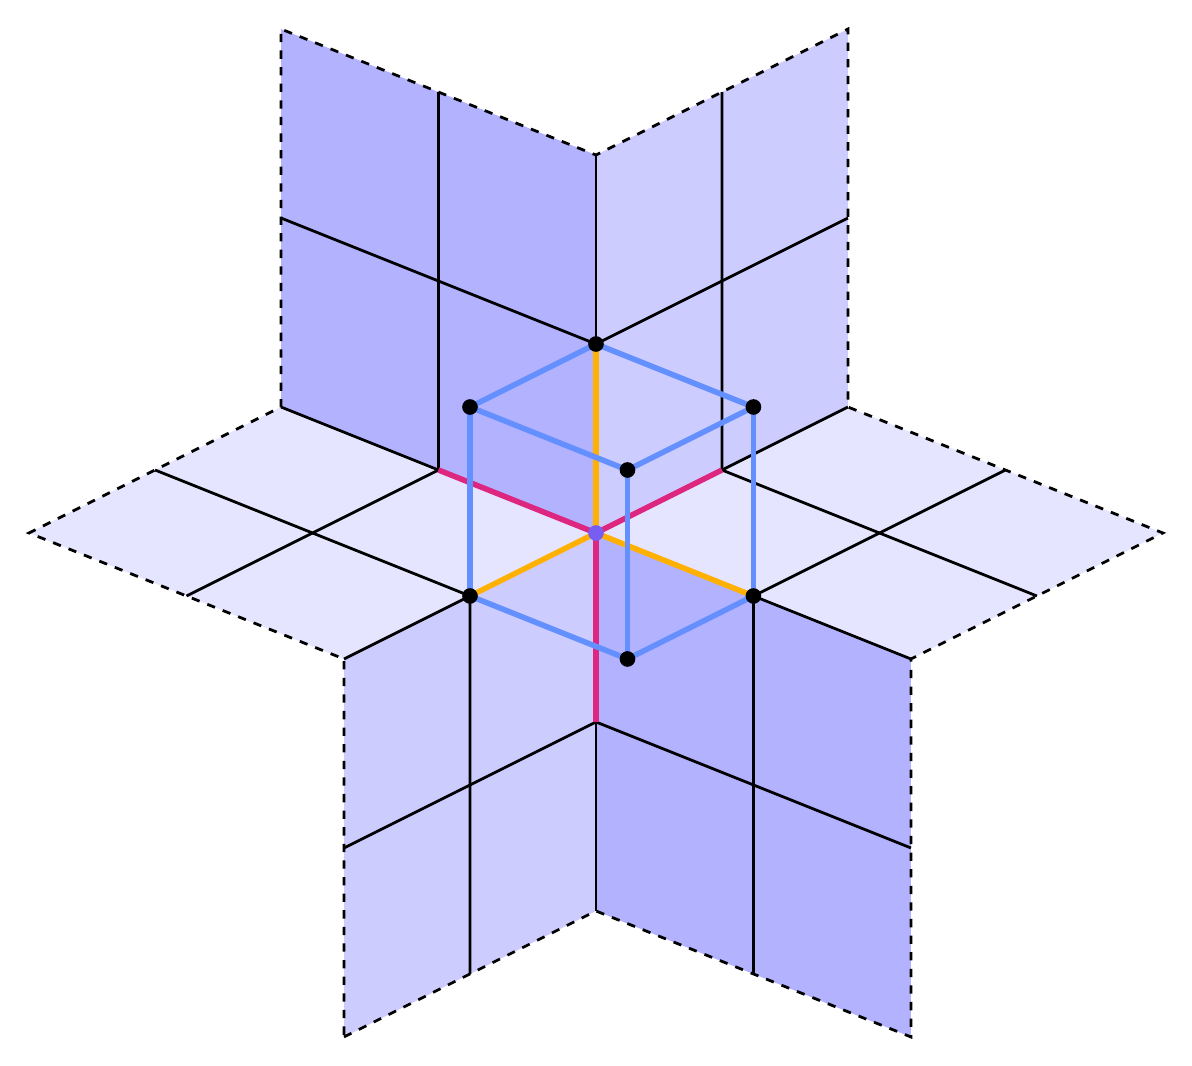
\begin{tikzpicture}[scale=4, x={(0.5cm,-0.2cm)}, y={(0.4cm,0.2cm)}, z={(0.0cm,0.6cm)}]

  %%%%%%%%%% Points pour travailler %%%%%%%%%%

 \coordinate (0) at (0,-2,-2);
 \coordinate (1) at (0,-1,-2);
 \coordinate (2) at (0,0,-2);
 \coordinate (3) at (1,0,-2);
 \coordinate (4) at (2,0,-2);
 \coordinate (5) at (0,-2,-1);
 \coordinate (6) at (0,-1,-1);
 \coordinate (7) at (0,0,-1);
 \coordinate (8) at (1,0,-1);
 \coordinate (9) at (2,0,-1);
 \coordinate (10) at (-2,-2,0);
 \coordinate (11) at (-2,-1,0);
 \coordinate (12) at (-2,0,0);
 \coordinate (13) at (-1,-2,0);
 \coordinate (14) at (-1,-1,0);
 \coordinate (15) at (-1,0,0);
 \coordinate (16) at (0,-2,0);
 \coordinate (17) at (0,-1,0);
 \coordinate (18) at (0,0,0);
 \coordinate (19) at (0,1,0);
 \coordinate (20) at (0,2,0);
 \coordinate (21) at (1,-1,0);
 \coordinate (22) at (1,0,0);
 \coordinate (23) at (1,1,0);
 \coordinate (24) at (1,2,0);
 \coordinate (25) at (2,0,0);
 \coordinate (26) at (2,1,0);
 \coordinate (27) at (2,2,0);
 \coordinate (28) at (-2,0,1);
 \coordinate (29) at (-1,0,1);
 \coordinate (30) at (0,-1,1);
 \coordinate (31) at (0,0,1);
 \coordinate (32) at (0,1,1);
 \coordinate (33) at (0,2,1);
 \coordinate (34) at (1,-1,1);
 \coordinate (35) at (1,0,1);
 \coordinate (36) at (-2,0,2);
 \coordinate (37) at (-1,0,2);
 \coordinate (38) at (0,0,2);
 \coordinate (39) at (0,1,2);
 \coordinate (40) at (0,2,2);

 
 %%%%%%%%%% Layer blue color %%%%%%%%%%
 \fill [color=blue!30!white] (18) -- (38) -- (36) -- (12) -- cycle ;
 \fill [color=blue!30!white] (18) -- (25) -- (4) -- (2) -- cycle ;
 \fill [color=blue!20!white] (18) -- (20) -- (40) -- (38) -- cycle ;
 \fill [color=blue!20!white] (18) -- (16) -- (0) -- (2) -- cycle ;
 \fill [color=blue!10!white] (18) -- (12) -- (10) -- (16) -- cycle ;
 \fill [color=blue!10!white] (18) -- (20) -- (27) -- (25) -- cycle ;
 
 %%%%%%%%%%%%%%%% Precedant layer %%%%%%%%%%%%%%%%%%%
 \draw [line width=1] (12) -- (25) ;
 \draw [line width=1] (16) -- (20) ;
 \draw [line width=1] (38) -- (2) ;

 \draw [line width=1] (11) -- (17) -- (1) ;
 \draw [line width=1] (28) -- (31) -- (33) ;
 \draw [line width=1] (3) -- (22) -- (24) ;
 \draw [line width=1] (13) -- (15) -- (37) ;
 \draw [line width=1] (5) -- (7) -- (9) ;
 \draw [line width=1] (39) -- (19) -- (26) ;

 \draw [dashed, line width=1] (0) -- (2) -- (4) -- (25) -- (27) -- (20) -- (40) -- (38) -- (36) -- (12) -- (10) -- (16) -- (0) ;
 
 
 %%%%%%%%%%% Feature edges %%%%%%%%%%%
 \draw [line width=2, color=End] (18) -- (15) ;
 \draw [line width=2, color=End] (18) -- (7) ;
 \draw [line width=2, color=End] (18) -- (19) ;
 \draw [line width=2, color=Corner] (18) -- (31) ;
 \draw [line width=2, color=Corner] (18) -- (17) ;
 \draw [line width=2, color=Corner] (18) -- (22) ;

 %%%%%%%%%%% Faces %%%%%%%%%%%
 \draw [opacity=0] (18) -- (29) ;
 \draw [opacity=0] (18) -- (14) ;
 \draw [opacity=0] (18) -- (6) ;
 \draw [opacity=0] (18) -- (8) ;
 \draw [opacity=0] (18) -- (23) ;
 \draw [opacity=0] (18) -- (32) ;
 
 
 %%%%%%%%%%% The HEXA created %%%%%%%%%%% 
 \draw [line width=2, color=NewHex] (30) -- (31) -- (35) -- (34) -- (30) ;
 \draw [line width=2, color=NewHex] (17) -- (21) -- (22) ;
 \draw [line width=2, color=NewHex] (30) -- (17) ;
 \draw [line width=2, color=NewHex] (34) -- (21) ;
 \draw [line width=2, color=NewHex] (35) -- (22) ;

  %%%%%%%%%%% HEXA NODES %%%%%%%%%%%
 \draw (18) node[circle, fill=n0, inner sep = 2 pt] {};
 \draw (17) node[circle, fill=black, inner sep = 2 pt] {};
 \draw (21) node[circle, fill=black, inner sep = 2 pt] {};
 \draw (22) node[circle, fill=black, inner sep = 2 pt] {};
 \draw (30) node[circle, fill=black, inner sep = 2 pt] {};
 \draw (31) node[circle, fill=black, inner sep = 2 pt] {};
 \draw (34) node[circle, fill=black, inner sep = 2 pt] {};
 \draw (35) node[circle, fill=black, inner sep = 2 pt] {};

\end{tikzpicture}
\end{document}